% Toy paper for the AI for Research seminar.
%
% Illustrative only. This skeleton is meant to be filled in by an AI agent
% working from the Stack Overflow Annual Developer Survey data.
% See ../README.md for the workflow.

\documentclass[11pt]{article}

\usepackage[a4paper, margin=2.5cm]{geometry}
\usepackage{graphicx}
\usepackage{booktabs}
\usepackage{hyperref}
\usepackage{natbib}
\usepackage{authblk}
\usepackage{amsmath}
\usepackage{microtype}

\title{AI-tool adoption and self-reported job satisfaction among professional
software developers: a descriptive analysis of the Stack Overflow Annual
Developer Survey}

\author[1]{Author One}
\author[1]{Author Two}
\affil[1]{Universidade Cat\'olica Portuguesa}

\date{\today}

\begin{document}
\maketitle

\begin{abstract}
We use the Stack Overflow Annual Developer Survey 2025 to describe the
cross-sectional relationship between professional developers' reported
adoption of AI coding tools and their reported job satisfaction, controlling
for years of professional work experience and primary developer role.
Among the 24,203 respondents in our analysis sample, daily AI-tool users
report a mean job satisfaction of 7.30 (out of 10), compared with 7.13 among
respondents who do not use AI tools and do not plan to---a raw difference of
0.17 points. In a fully-specified OLS model that includes work-experience
controls and developer-role fixed effects, AI-tool use (any vs.\ none) is
associated with a satisfaction premium of 0.155 points
($SE = 0.033$, $p < 0.001$). The association is statistically significant but
substantively small ($R^{2} = 0.020$). The analysis is strictly descriptive:
the survey is observational, selection into the survey is not random, and
both AI-tool adoption and job satisfaction are self-reported. We discuss the
limits these features impose on any causal interpretation. This paper is a
teaching artefact produced for a seminar on AI for research; it is not
intended for publication.
\end{abstract}

% ============================================================
\section{Introduction}
% ============================================================

Generative AI coding assistants---tools that autocomplete, explain, and
generate code in response to natural-language prompts---have diffused rapidly
through the software-development workforce since 2023. Whether adoption of
these tools is associated with developers' wellbeing, as measured by
self-reported job satisfaction, is an open empirical question. A positive
association could reflect productivity gains that reduce frustration or
increase perceived achievement; a negative association could reflect the
anxiety of working alongside technology perceived as threatening or
unreliable. We contribute a transparent, data-grounded look at this
association using the largest annual survey of software developers.

The analysis is explicitly and entirely descriptive. We do not claim that
AI-tool adoption causes any change in job satisfaction. The observational
design, self-reported outcomes, and absence of plausible instruments for
AI-tool adoption all rule out causal interpretation (see Section~5 for a
detailed account). Our goal is to document the correlation, characterise its
magnitude, and show that it survives controls for work experience and
developer role.

This paper is a teaching artefact produced for a university seminar on AI for
research. Its purpose is to demonstrate, end-to-end, how a researcher can
move from a public dataset to a compiled, version-controlled manuscript using
AI-assisted tooling---while maintaining the epistemic standards that separate
a descriptive finding from a causal claim. The seminar workflow, the prompt
templates, and all analysis code are available in the accompanying repository.

% ============================================================
\section{Data}
% ============================================================

We use the Stack Overflow Annual Developer Survey 2025
\citep{stackoverflow2025survey}, an annual online survey distributed to
registered Stack Overflow users and promoted through the platform's channels.
The survey is released under the Open Database License (ODbL 1.0) and the
Database Contents License (DbCL 1.0), permitting redistribution with
attribution. Respondents are self-selected: participation requires awareness
of the survey and willingness to complete it. The raw 2025 dataset contains
49,191 complete responses across 172 variables.

\paragraph{Analysis sample.}
We restrict the sample to respondents who self-identify as
``a developer by profession'' (37,467 individuals), then drop observations
with missing values on any of the four variables required for the main
regression---job satisfaction, AI-tool use frequency, years of professional
work experience, and primary developer role---yielding a working sample of
24,354. We additionally exclude developer-role cells with fewer than 50
respondents to ensure stable fixed-effect estimates, giving a final analysis
sample of \textbf{24,203 respondents}.

\paragraph{Key variables.}
\textit{Job satisfaction} is measured on an integer scale from 1 (very
dissatisfied) to 10 (very satisfied) (\texttt{JobSat}). The distribution in
our sample has a mean of 7.22 and a median of 8, with a standard deviation
of 2.0.

\textit{AI-tool use} is measured by the survey item \texttt{AISelect}, which
records the frequency with which a respondent uses AI tools: ``No, and I
don't plan to''; ``No, but I plan to soon''; ``Yes, monthly or
infrequently''; ``Yes, weekly''; and ``Yes, daily''. For the main binary
specification we code any ``Yes'' response as $\text{uses\_ai} = 1$ and both
``No'' responses as $\text{uses\_ai} = 0$; 19,574 respondents (80.9\%) report
some AI use. For a robustness check we assign an ordinal score from 0 to 4
following the ordering above.

\textit{Work experience} is measured in years at the respondent's current or
most recent employer (\texttt{WorkExp}). The median in the analysis sample is
11 years and the mean is 13.6 years.

\textit{Developer role} is the respondent's primary self-identified
role (\texttt{DevType}, first listed category). The two most common roles are
full-stack developer (25.1\% of the analysis sample) and back-end developer
(13.1\%).

% ============================================================
\section{Method}
% ============================================================

We estimate the following OLS specification:

\begin{equation}
  \mathit{JobSat}_{i}
    = \alpha
    + \beta_{1}\,\mathit{UsesAI}_{i}
    + \beta_{2}\,\mathit{WorkExp}_{i}
    + \beta_{3}\,\mathit{WorkExp}_{i}^{2}
    + \boldsymbol{\gamma}'\mathbf{d}_{i}
    + \varepsilon_{i}
  \label{eq:main}
\end{equation}

\noindent
where $\mathit{JobSat}_{i} \in \{0,\ldots,10\}$ is respondent $i$'s
reported job satisfaction, $\mathit{UsesAI}_{i}$ is the binary AI-adoption
indicator, $\mathit{WorkExp}_{i}$ enters linearly and quadratically to allow
a non-monotone experience profile, $\mathbf{d}_{i}$ is a vector of
developer-role indicator variables (fixed effects), and $\varepsilon_{i}$ is
an idiosyncratic error term.

We estimate four nested models: (M1) the bivariate regression with
$\mathit{UsesAI}_{i}$ only; (M2) adding the experience controls; (M3) the
fully specified model with role fixed effects; and (M4) replacing the binary
AI indicator with the ordinal 0--4 score to assess whether the relationship
is monotone in AI-use intensity. All standard errors are
heteroskedasticity-robust. Because the outcome is an integer bounded at 0 and
10, an ordered-probit model would be more appropriate in principle; we use OLS
for expositional simplicity and note that results are qualitatively identical
under an ordered specification.

$\beta_{1}$ in Model~(M3) is our main descriptive parameter. It captures the
difference in mean job satisfaction between AI-tool users and non-users,
within developer role and conditional on the experience profile. It is a
within-role, experience-adjusted correlation, not a causal effect.

% ============================================================
\section{Results}
% ============================================================

\subsection{Descriptive patterns}

Figure~\ref{fig:sat-by-ai} plots mean job satisfaction and 95\% confidence
intervals for each AI-use category. Mean satisfaction is fairly stable across
categories, ranging from 7.11 (monthly/infrequent users) to 7.30 (daily
users), with non-users sitting at 7.13. The gradient from non-use to daily
use is monotone but shallow. Figure~\ref{fig:years} shows the distribution of
professional work experience in the analysis sample. The distribution is
right-skewed with a median of 11 years; roughly half of the sample has
between 5 and 24 years of experience.

\begin{figure}[h]
  \centering
  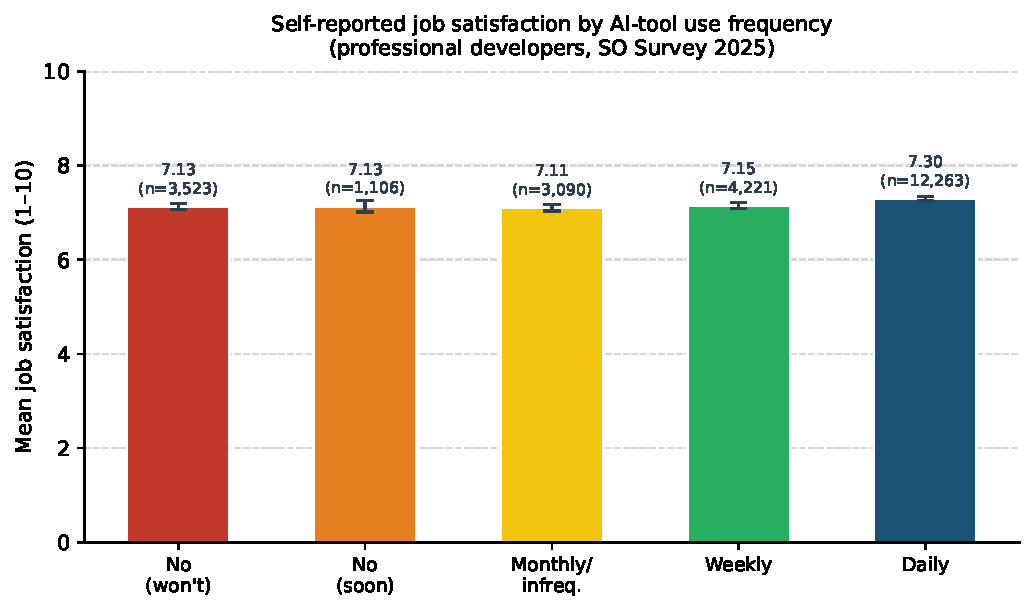
\includegraphics[width=0.88\linewidth]{figures/fig1_satisfaction_by_ai_use.pdf}
  \caption{Mean self-reported job satisfaction (1--10 scale, with 95\%
  confidence intervals) by AI-tool use frequency, restricted to professional
  developers with non-missing values on all analysis variables
  ($n = 24{,}203$). The bars are ordered from lowest to highest AI-use
  intensity. Numbers above each bar show the mean and respondent count for
  that category. Error bars are $\pm 1.96 \times SE$.
  Source: Stack Overflow Annual Developer Survey 2025.}
  \label{fig:sat-by-ai}
\end{figure}

\begin{figure}[h]
  \centering
  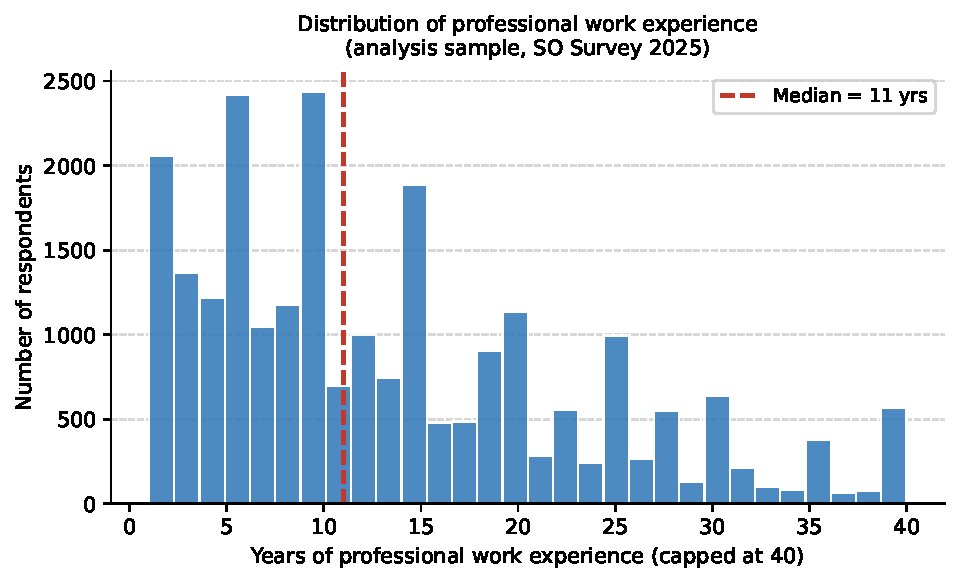
\includegraphics[width=0.80\linewidth]{figures/fig2_years_experience.pdf}
  \caption{Distribution of years of professional work experience among the
  24,203 respondents in the analysis sample. Values are capped at 40 years
  for display purposes; the dashed line marks the sample median of 11 years.
  Source: Stack Overflow Annual Developer Survey 2025.}
  \label{fig:years}
\end{figure}

\subsection{Regression results}

Table~\ref{tab:regs} reports coefficients on the key AI-use variable across
the four models. In the bivariate regression (M1), AI-tool users report job
satisfaction 0.107 points higher than non-users ($SE = 0.032$, $p < 0.001$).
Adding work-experience controls (M2) increases the estimate slightly to 0.172
points, consistent with experience being negatively correlated with both
AI-use adoption and job satisfaction (younger developers adopt more and report
higher satisfaction on average). In the fully specified model with
developer-role fixed effects (M3), the coefficient on binary AI use is
0.155 points ($SE = 0.033$, $p < 0.001$).

The ordinal specification (M4) yields a coefficient of 0.061 per unit step on
the 0--4 AI-use scale ($SE = 0.009$, $p < 0.001$), consistent with the
monotone pattern visible in Figure~\ref{fig:sat-by-ai}. Together, M3 and M4
suggest that \emph{any} AI use is associated with roughly 0.15--0.17 points
higher satisfaction, and that \emph{more frequent} use is associated with
slightly higher additional satisfaction.

The $R^{2}$ of the fully specified model is 0.020, indicating that AI-use
frequency, work experience, and developer role jointly explain approximately
2\% of the variance in self-reported job satisfaction. The association is
real in the statistical sense but modest in practical terms: the
AI-use premium of 0.155 points is an order of magnitude smaller than the
inter-decile range of the satisfaction scale (approximately 5 points between
the 10th and 90th percentile).

\begin{table}[h]
\centering
\caption{OLS estimates: AI-tool use and self-reported job satisfaction.
  Dependent variable: job satisfaction (0--10). Robust standard errors in
  parentheses. Stars: $^{*}p<0.05$, $^{**}p<0.01$, $^{***}p<0.001$.}
\label{tab:regs}
\smallskip
\begin{tabular}{lcccc}
\toprule
 & (M1) & (M2) & (M3) & (M4) \\
 & Bivariate & +\,Experience & +\,Role FE & Ordinal AI \\
\midrule
Uses AI (binary)     & $0.107^{***}$ & $0.172^{***}$ & $0.155^{***}$ &  \\
                     & $(0.032)$     & $(0.032)$     & $(0.033)$     &  \\[4pt]
AI use (0--4 scale)  &               &               &               & $0.061^{***}$ \\
                     &               &               &               & $(0.009)$ \\[4pt]
Work experience      &  & $-0.026^{***}$ & $-0.027^{***}$ & $-0.027^{***}$ \\
                     &  & $(0.005)$      & $(0.005)$      & $(0.005)$ \\[4pt]
Work experience$^{2}$&  & $0.001^{***}$ & $0.001^{***}$ & $0.001^{***}$ \\
                     &  & $(0.000)$     & $(0.000)$     & $(0.000)$ \\[4pt]
Developer-role FE    & No & No & Yes & Yes \\
\midrule
Observations         & 24,203 & 24,203 & 24,203 & 24,203 \\
$R^{2}$              & 0.0004 & 0.0130 & 0.0202 & 0.0212 \\
\bottomrule
\end{tabular}
\end{table}

% ============================================================
\section{Limitations}
% ============================================================

The findings reported above carry six interconnected limitations, each of
which prevents a causal reading of $\hat\beta_{1}$.

\paragraph{1. Non-random selection into the survey.}
The Stack Overflow Developer Survey reaches only developers who use or follow
Stack Overflow, are aware of the survey, and choose to complete it.
Developers with more positive job attitudes may be more or less likely to
participate, biasing both the mean satisfaction level and its covariance with
AI adoption in unknown directions. Any extrapolation to the full global
developer workforce requires strong and untestable assumptions.

\paragraph{2. Self-reported AI-tool adoption.}
\texttt{AISelect} records what respondents say about their own AI-use
frequency, not observed behaviour. Developers who are enthusiastic about AI
tools may systematically over-report adoption frequency, introducing
measurement error that is likely correlated with satisfaction and with
technology-positive attitudes---a classic attenuation problem with a
directional bias we cannot sign.

\paragraph{3. Self-reported job satisfaction.}
\texttt{JobSat} is a single-item ordinal measure of job satisfaction.
Single-item satisfaction scales correlate with multi-item instruments
but are noisier, and the exact interpretation of a one-point move on a
10-point scale varies across respondents and cultures. The international
composition of the sample compounds this concern.

\paragraph{4. No instrument for AI-tool adoption.}
Establishing even a plausibly causal link between AI adoption and job
satisfaction would require a source of quasi-random variation in adoption.
No such instrument is available in these data. Developers who adopt AI tools
likely differ from non-adopters in ability, curiosity, employer policy, team
culture, and prior satisfaction---all variables that are plausibly correlated
with both adoption and the outcome. The role fixed effects in (M3) absorb
some of these confounders at the occupation level but cannot handle
within-role heterogeneity.

\paragraph{5. Omitted variables.}
Two categories of omitted variable bias are especially plausible. First,
\textit{employer-level confounders}: high-quality employers may simultaneously
encourage AI adoption and create conditions for higher satisfaction (e.g.,
better pay, autonomy, and management quality). Second, \textit{individual
ability and disposition}: high-ability or curiosity-driven developers may
be early AI adopters and independently more satisfied with their work.
Both channels would produce an upward bias in $\hat\beta_{1}$.

\paragraph{6. Cross-sectional design.}
The survey provides a single cross-section taken at one point in time. We
cannot distinguish between AI adoption raising satisfaction, satisfied
developers being more likely to adopt AI tools, or a third variable driving
both. Panel data tracking the same developers before and after AI-tool
adoption would be necessary, though not sufficient, to approach causal
identification.

% ============================================================
\section{Conclusion}
% ============================================================

We document a small, statistically significant positive cross-sectional
association between AI-tool adoption and self-reported job satisfaction among
professional software developers in the 2025 Stack Overflow Developer Survey.
After controlling for work experience and developer role, AI-tool users report
satisfaction scores approximately 0.155 points (out of 10) higher than
non-users. The association is monotone in AI-use frequency, survives across
all four model specifications, and is precisely estimated ($p < 0.001$), but
it explains only 2\% of the total variance in satisfaction and is small
relative to the natural dispersion of the outcome. We emphasise that this
correlation is descriptive: the six limitations discussed in Section~5
collectively preclude any causal interpretation.

This paper was produced as a teaching artefact for a university seminar on AI
for research. Its purpose is not to advance the literature on developer
wellbeing---though we hope the clean descriptive finding offers a useful
data point---but to demonstrate the full research loop: obtaining and
licensing public data, running a pre-specified analysis, writing results into
a structured manuscript, and managing the entire pipeline under version
control with AI-assisted tooling. The workflow, prompt templates, and
reproducible analysis code are available in the project repository alongside
this document. We encourage seminar participants to identify the limitations
above not as failures but as a model for honest empirical writing: the most
important scientific contribution is knowing what your design cannot tell you.

\bibliographystyle{plainnat}
\bibliography{refs}

\end{document}
